\chapter{Datasets}
\label{datasets}

\resetfigpath{2-datasets}
This chapter describes the datasets considered in the present thesis.
Tab. \ref{tab:dataset_stat} summarizes the 4 dataset types.
We used four different MRI brain sequences (A-D).
To augment the number of images for one dataset, the last three datasets (B-D) are combined into one larger dataset \textit{MRI Brain (B-D)}.
In a similar manner, dataset \textit{Slit-Lamp Retina (A-D)} is constructed from concatenating four independent datasets together.
The two independent datasets of the inner ear CT could not be concatenated due to different image resolutions.

\begin{table}
\centering
\caption{
    Overview of datasets.
    }
\label{tab:dataset_stats}
\begin{tabular}{llp{1.8cm}p{1.8cm}p{1.8cm}p{1.8cm}p{1.8cm}}
\toprule
      &   &  Height &  Width &   Color \\
\midrule
\multirow{4}{*}{Tweezer} & A &     576 &    720 &  \cmark \\
      & B &     576 &    720 &  \cmark \\
      & C &     576 &    720 &  \cmark \\
      & D &     576 &    720 &  \cmark \\
\cline{1-5}
\multirow{4}{*}{Cochlea} & A &     546 &    720 &  \xmark \\
      & B &     546 &    720 &  \xmark \\
      & C &     546 &    720 &  \xmark \\
      & D &     546 &    720 &  \xmark \\
\cline{1-5}
\multirow{4}{*}{Slitlamp} & A &     512 &    680 &  \cmark \\
      & B &     512 &    680 &  \cmark \\
      & C &     512 &    680 &  \cmark \\
      & D &     512 &    680 &  \cmark \\
\cline{1-5}
\multirow{4}{*}{Brain} & A &     540 &    782 &  \xmark \\
      & B &     559 &    561 &  \xmark \\
      & C &     559 &    561 &  \xmark \\
      & D &     559 &    561 &  \xmark \\
\bottomrule
\end{tabular}
\end{table}


\begin{figure}
\centering
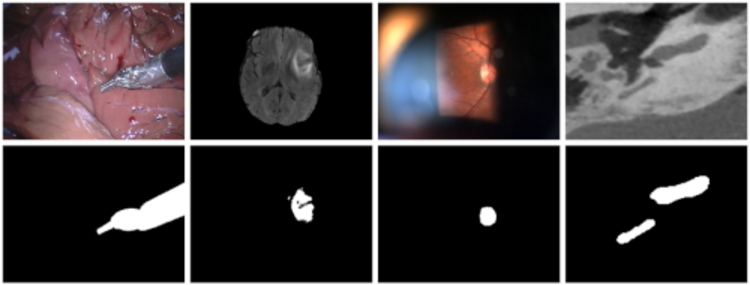
\includegraphics[width=0.99\textwidth]{previews.pdf}
\caption{Example of objects of interest in different video and volumetric modalities. The bottom row shows the pixel wise segmentation for each case: From left to right: A surgical instrument during an endoscopic procedure, a 3D MRI scan containing a brain tumor, an optic disc seen from a slit lamp microscope and a cochlea cross-section in a 3D CT scan.}
\label{fig:dset_previews}
\end{figure}

%%% Local Variables:
%%% mode: latex
%%% TeX-master: "../../main"
%%% End:
